\chapter{Acasxu verification}
\label{chap:ch3}

\par To ensure the reliability and safety of Acasxu, a verification was employed using Alpha-Beta-CROWN. This tool relies on data from two files: a VNNLIB file outlining the property to be verified and a file containing the neural network in an ONNX format. Its goal is to test whether the specified property holds true for the given neural network and input constraints. 

\par Initially, the testing focused solely on property 1 to gain insights into the output. This output contains details about configuration, attack parameters, model output, properties, verification iterations, results, and a summary. Every iteration provides data about the batch size, the worst lower bound encountered, the total time spent in that iteration, the number of domains or branches explored, the cumulative time and the current lower bound - right-hand side value. This particular value is used to asses whether the property is satisfied or not, since a negative value indicates a potential violation of the property. One example of such iteration can be observed in figure \ref{Fig_It1}.

\begin{figure}[htbp]
	\centering
		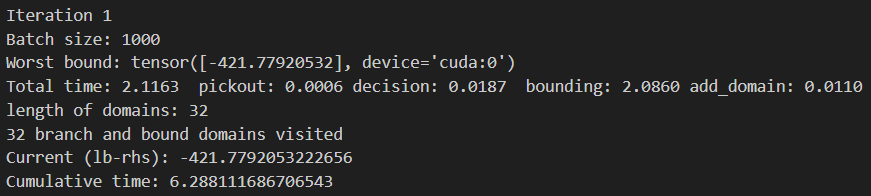
\includegraphics[width=12cm]{./Figures/it1.png}
	\caption{Iteration 1}
	\label{Fig_It1}
\end{figure}

\par The summary provides an overview of the verification progress. In the case of the first property tested, the verification concluded in 24.8 seconds. Its summary can be seen in figure \ref{Fig_Summary1}. The tool successfully checked that no safety violations were found within the specified property constraints with an accuracy of 100\% and a mean time of approximately 24.87 seconds.

\begin{figure}[htbp]
	\centering
		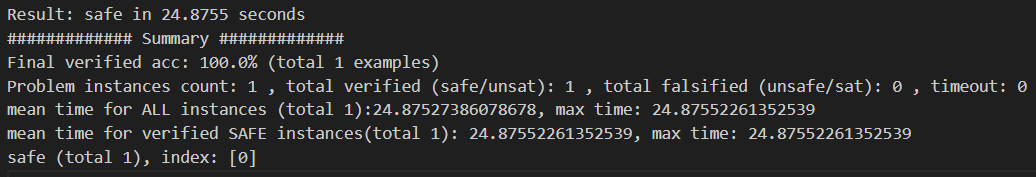
\includegraphics[width=12cm]{./Figures/summary1.png}
	\caption{Summary for property 1}
	\label{Fig_Summary1}
\end{figure}

\par The next phase involved testing all properties, aiming to evaluate the neural network's behavior across various configurations and constraints. The final verified accuracy stands at approximately 74.73\%. Out of the 186 instances tested, 139 were verified as safe, meaning that the property held true. There was 1 instance that resulted in a timeout, indicating an inconclusive verification process. In terms of verification times, the mean time taken for verifying all instances was approximately 3.43 seconds, with the maximum time being around 121.67 seconds. Regarding the branch and bound method (BAB), 4 instances were marked as unsafe, whereas in the context of the Projected Gradient Descent (PGD) method, 42 instances were identified as unsafe. Additionally, one instance fell into an unknown category, likely meaning it couldn't be clearly classified as safe or unsafe. All of this information, along with more detailed insights, can be observed in figure \ref{Fig_Summary}.

\begin{figure}[htbp]
	\centering
		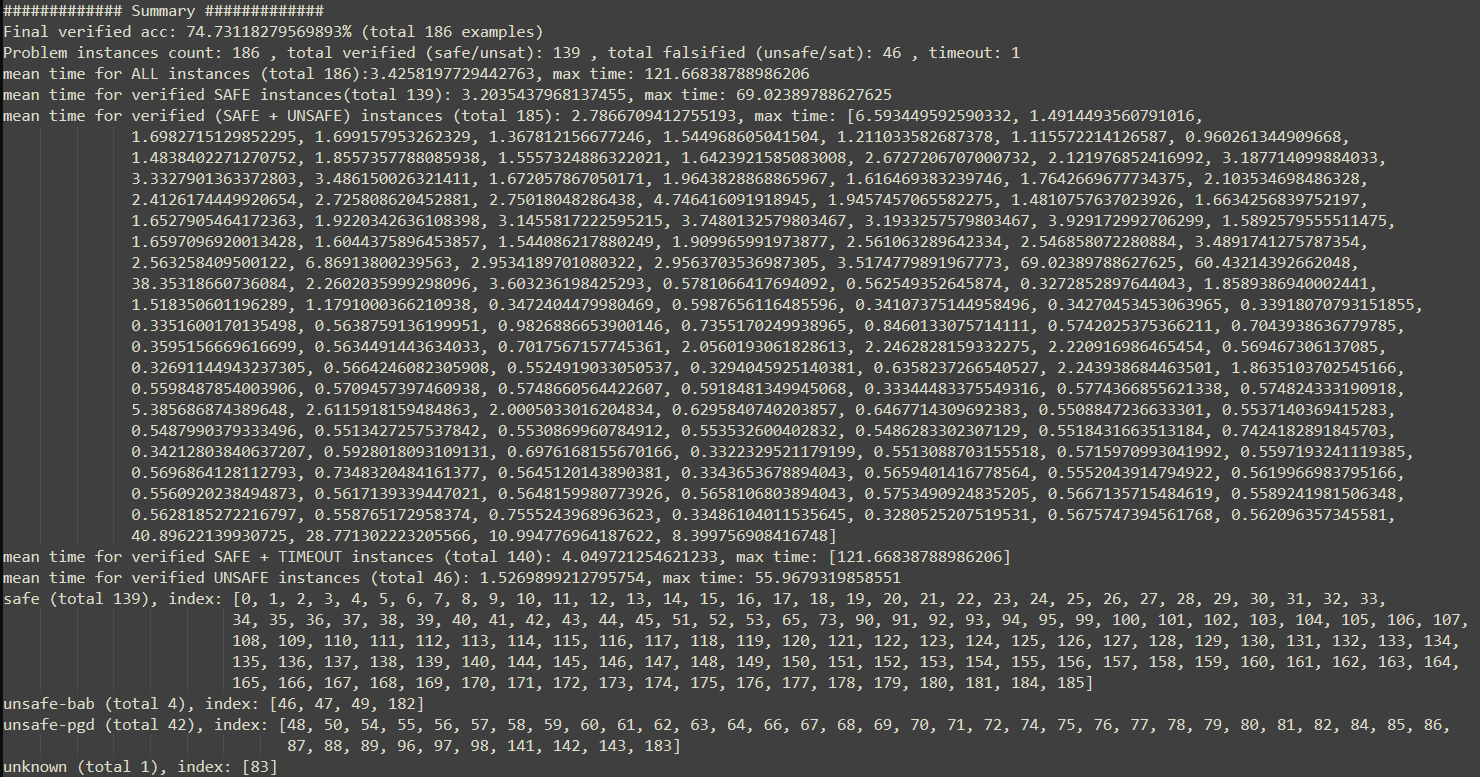
\includegraphics[width=15cm]{./Figures/summary.png}
	\caption{Summary}
	\label{Fig_Summary}
\end{figure}